\documentclass[12pt,a4paper,fleqn]{article}
\usepackage[utf8]{inputenc}
\usepackage[russian]{babel}
\usepackage{amssymb, amsmath, multicol}
\usepackage{enumitem}
\usepackage{lipsum}
\usepackage{euler}
\oddsidemargin=-15.4mm
\textwidth=190mm
\headheight=-32.4mm
\textheight=277mm
\parindent=0pt
\parskip=8pt
\pagestyle{empty}
\usepackage{graphicx}
\title{\textbf{\LARGE{Исследовательская работа по теме:\\Исследование функции дифференциальными методами}}}
\author{Известный гражданин}
\date{November 2022}
\addt\captionsrussian{\def\refname{Список литературы}}\begin{document}
\maketitle
\newpage\newpage \textbf{\LARGE{Глава I. Функция}}

\begin{center}
$y = $$sin((cos(x))^{2})$

\end{center}
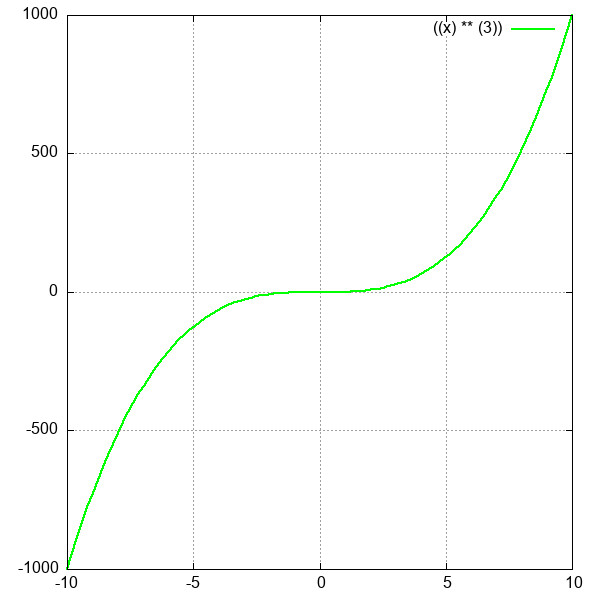
\includegraphics{GraphicDumps/plot.jpg}\newpage \textbf{\LARGE{Глава II. Визуальный анализ функции}}

Так как 1=1, то\cite{link4}

\begin{center}
$y = $$sin((cos(x))^{2})$

\end{center}
\newpage \textbf{\LARGE{Глава III. Дифференцирование}}

Дифференциал от производной не далеко падает\cite{link2}

\begin{center}
 ($x)'
  = 1$\end{center}
Доказательство данного факта предоставлено лицом или организацией исполняющей функции иностанного агента

\begin{center}
 ($cos(x))'
  = 1 \cdot 0-sin(x)$\end{center}
Здесь могла быть ваша реклама

\begin{center}
A = $(2-1) \cdot (cos(x))^{2-1}$\end{center}
\begin{center}
 ($(cos(x))^{2})'
  = (A) \cdot 1 \cdot 0-sin(x)$\end{center}
Положим

\begin{center}
A = $(2-1) \cdot (cos(x))^{2-1}$\end{center}
\begin{center}
 ($sin((cos(x))^{2}))'
  = ((A) \cdot 1 \cdot 0-sin(x)) \cdot cos((cos(x))^{2})$\end{center}
DUMP

$(((2-1) \cdot (cos(x))^{2-1}) \cdot 1 \cdot 0-sin(x)) \cdot cos((cos(x))^{2})$DUMP
\newpage \textbf{\LARGE{Глава IV.Упрощение выражения}}

Производная дураков любит\cite{link2}

\begin{center}$2-1 = 1$\end{center}
Британские учёные доказали, что для поддержания мозга в тонусе необходимо ежедневно дифференцировать. Продолжим наше приобщение к здоровому образу жизниn

\begin{center}$2-1 = 1$\end{center}
Телец в козероге, поэтому

\begin{center}
$(cos(x))^{1} = cos(x)$\end{center}
Я придумал поистине удивительное доказательство этого факта, но поля этой книги слишком малы\ldots

\begin{center}
$1 \cdot cos(x) = cos(x)$\end{center}
Вы не шокированы?\cite{link3}

\begin{center}
$1 \cdot 0-sin(x) = 0-sin(x)$\end{center}
\newpage \textbf{\LARGE{Глава V. Полученая производная}}

$y = $$sin((cos(x))^{2})$

\begin{center}
A = $cos(x) \cdot 0-sin(x)$\end{center}
$y' = $$(A) \cdot cos((cos(x))^{2})$

\includegraphics{GraphicDumps/plot_1.jpg}\newpage \textbf{\LARGE{Глава VI. Разложение функции по формуле Тейлора}}

Если посмотреть на выражение под другим углом, можно получить

\begin{center}$cos(0) = 1$\end{center}
Производная дураков любит\cite{link2}

\begin{center}$1^{2} = 1$\end{center}
[Данные удалены]

\begin{center}$sin(1) = 0.841471$\end{center}
Функция производной не стоит\cite{link2}

\begin{center}
 ($x)'
  = 1$\end{center}
Британские учёные доказали, что для поддержания мозга в тонусе необходимо ежедневно дифференцировать. Продолжим наше приобщение к здоровому образу жизниn

\begin{center}
 ($cos(x))'
  = 1 \cdot 0-sin(x)$\end{center}
Если посмотреть на выражение под другим углом, можно получить

\begin{center}
A = $(2-1) \cdot (cos(x))^{2-1}$\end{center}
\begin{center}
 ($(cos(x))^{2})'
  = (A) \cdot 1 \cdot 0-sin(x)$\end{center}
С другой стороны

\begin{center}
A = $(2-1) \cdot (cos(x))^{2-1}$\end{center}
\begin{center}
 ($sin((cos(x))^{2}))'
  = ((A) \cdot 1 \cdot 0-sin(x)) \cdot cos((cos(x))^{2})$\end{center}
Обоснование этого пререхода предостовляется читателю в качестве несложного упрожнения

\begin{center}$2-1 = 1$\end{center}
Я придумал поистине удивительное доказательство этого факта, но поля этой книги слишком малы\ldots

\begin{center}$2-1 = 1$\end{center}
Очевидно, что

\begin{center}
$(cos(x))^{1} = cos(x)$\end{center}
Обоснование этого пререхода предостовляется читателю в платном DLC

\begin{center}
$1 \cdot cos(x) = cos(x)$\end{center}
Нам не объяснили на семинаре как это делать, поэтому примем на веру

\begin{center}
$1 \cdot 0-sin(x) = 0-sin(x)$\end{center}
По теореме Эскобара

\begin{center}$cos(0) = 1$\end{center}
Дураку понятно, что

\begin{center}$sin(0) = 0$\end{center}
Кроме того

\begin{center}$0-0 = 0$\end{center}
(null)\cite{link4}

\begin{center}$1 \cdot 0 = 0$\end{center}
Без комментариев\cite{link4}

\begin{center}$cos(0) = 1$\end{center}
По лемме $\sqrt{-759}$
\begin{center}$1^{2} = 1$\end{center}
Вы не шокированы?\cite{link3}

\begin{center}$cos(1) = 0.540302$\end{center}
Ты же продолжаешь читать, да?

\begin{center}$0 \cdot 0.540302 = 0$\end{center}
Автору приснилось, что следующее преобразование верно

\begin{center}
$x-0 = x$\end{center}
Я придумал поистине удивительное доказательство этого факта, но поля этой книги слишком малы\ldots

\begin{center}
$x^{1} = x$\end{center}
ИИИИЕЕЕЕсли\cite{link3}

\begin{center}
 ($x)'
  = 1$\end{center}
Функция производной не стоит\cite{link2}

\begin{center}
 ($cos(x))'
  = 1 \cdot 0-sin(x)$\end{center}
Производная дураков любит\cite{link2}

\begin{center}
 ($0)'
  = 0$\end{center}
(null)\cite{link4}

\begin{center}
 ($x)'
  = 1$\end{center}
Здесь могла быть ваша реклама

\begin{center}
 ($sin(x))'
  = 1 \cdot cos(x)$\end{center}
Если вы не понимаете этот переход, то я вам сочувствую

\begin{center}
 ($0-sin(x))'
  = 0-1 \cdot cos(x)$\end{center}
Здесь могла быть ваша реклама

\begin{center}
A = $(1 \cdot 0-sin(x)) \cdot 0-sin(x)$\end{center}
\begin{center}
B = $cos(x) \cdot 0-1 \cdot cos(x)$\end{center}
\begin{center}
 ($cos(x) \cdot 0-sin(x))'
  = A+B$\end{center}
Первая производная комом\cite{link2}

\begin{center}
 ($x)'
  = 1$\end{center}
Segmentation fault (core dumped)

\begin{center}
 ($cos(x))'
  = 1 \cdot 0-sin(x)$\end{center}
Не трудно заметить

\begin{center}
A = $(2-1) \cdot (cos(x))^{2-1}$\end{center}
\begin{center}
 ($(cos(x))^{2})'
  = (A) \cdot 1 \cdot 0-sin(x)$\end{center}
И хотя клуб любителей таких формул двумя блоками ниже, мы продолжаем

\begin{center}
A = $(2-1) \cdot (cos(x))^{2-1}$\end{center}
\begin{center}
B = $0-sin((cos(x))^{2})$\end{center}
\begin{center}
 ($cos((cos(x))^{2}))'
  = ((A) \cdot 1 \cdot 0-sin(x)) \cdot B$\end{center}
Производная дураков любит\cite{link2}

\begin{center}
A = $cos(x) \cdot 0-sin(x)$\end{center}
\begin{center}
B = $(1 \cdot 0-sin(x)) \cdot 0-sin(x)$\end{center}
\begin{center}
C = $cos(x) \cdot 0-1 \cdot cos(x)$\end{center}
\begin{center}
D = $(2-1) \cdot (cos(x))^{2-1}$\end{center}
\begin{center}
 ($(A) \cdot cos((cos(x))^{2}))'
  = (B+C) \cdot cos((cos(x))^{2})+(A) \cdot ((D) \cdot 1 \cdot 0-sin(x)) \cdot 0-sin((cos(x))^{2})$\end{center}
Я придумал поистине удивительное доказательство этого факта, но поля этой книги слишком малы\ldots

\begin{center}$2-1 = 1$\end{center}
Ну вот как этот матан тебе в жизни пригодится?

\begin{center}$2-1 = 1$\end{center}
Откуда

\begin{center}
$1 \cdot 0-sin(x) = 0-sin(x)$\end{center}
//TODO: Лёша, придумай переход. У меня идеи закончились

\begin{center}
$1 \cdot cos(x) = cos(x)$\end{center}
Имеем

\begin{center}
$(cos(x))^{1} = cos(x)$\end{center}
Если вы понимаете данный переход, то я вам сочувствую

\begin{center}
$1 \cdot cos(x) = cos(x)$\end{center}
Без комментариев\cite{link4}

\begin{center}
$1 \cdot 0-sin(x) = 0-sin(x)$\end{center}
Как будет доказано в следующем семестре

\begin{center}$sin(0) = 0$\end{center}
Британские учёные доказали, что для поддержания мозга в тонусе необходимо ежедневно дифференцировать. Продолжим наше приобщение к здоровому образу жизниn

\begin{center}$0-0 = 0$\end{center}
Автору приснилось, что следующее преобразование верно

\begin{center}$sin(0) = 0$\end{center}
Обоснование этого пререхода предостовляется читателю в качестве несложного упрожнения

\begin{center}$0-0 = 0$\end{center}
Автору приснилось, что следующее преобразование верно

\begin{center}$0 \cdot 0 = 0$\end{center}
Segmentation fault (core dumped)

\begin{center}$cos(0) = 1$\end{center}
\\ title{не сложно заметить} 

\begin{center}$cos(0) = 1$\end{center}
Так как 1=1, то\cite{link4}

\begin{center}$0-1 = -1$\end{center}
Если вы понимаете данный переход, то я вам сочувствую

\begin{center}$1 \cdot (-1) = -1$\end{center}
Обоснование этого пререхода предостовляется читателю в качестве несложного упрожнения

\begin{center}$0+(-1) = -1$\end{center}
Оказывается

\begin{center}$cos(0) = 1$\end{center}
Кроме того

\begin{center}$1^{2} = 1$\end{center}
Для любого эпсилон больше нулю очевидно, что

\begin{center}$cos(1) = 0.540302$\end{center}
Единственное, что я не понимаю, так это то, зачем ты это читаешь

\begin{center}$(-1) \cdot 0.540302 = -0.540302$\end{center}
Дефии... кхм, Дифири... тьфу ты, дифферин... Да что ж со мной такое сегодня? Дифференциал. Уф, совсем я заработался. Пойду отдохну *звук отодвигаемого стула, затем удаляющихся шагов*

\begin{center}$cos(0) = 1$\end{center}
Единственное, что я не понимаю, так это то, зачем ты это читаешь

\begin{center}$sin(0) = 0$\end{center}
Очевидно, что

\begin{center}$0-0 = 0$\end{center}
\\ title{не сложно заметить} 

\begin{center}$1 \cdot 0 = 0$\end{center}
Дефии... кхм, Дифири... тьфу ты, дифферин... Да что ж со мной такое сегодня? Дифференциал. Уф, совсем я заработался. Пойду отдохну *звук отодвигаемого стула, затем удаляющихся шагов*

\begin{center}$cos(0) = 1$\end{center}
Обоснование этого перехода было забанено редактурой

\begin{center}$sin(0) = 0$\end{center}
Дефии... кхм, Дифири... тьфу ты, дифферин... Да что ж со мной такое сегодня? Дифференциал. Уф, совсем я заработался. Пойду отдохну *звук отодвигаемого стула, затем удаляющихся шагов*

\begin{center}$0-0 = 0$\end{center}
\\ title{не сложно заметить} 

\begin{center}$1 \cdot 0 = 0$\end{center}
Дифференциал от производной не далеко падает\cite{link2}

\begin{center}$cos(0) = 1$\end{center}
Обоснование этого пререхода предостовляется читателю в качестве несложного упрожнения

\begin{center}$1^{2} = 1$\end{center}
Поэтому

\begin{center}$sin(1) = 0.841471$\end{center}
Отметим, что

\begin{center}$0-0.841471 = -0.841471$\end{center}
Оказывается

\begin{center}$0 \cdot (-0.841471) = -0$\end{center}
ИИИИЕЕЕЕсли\cite{link3}

\begin{center}$0 \cdot -0 = -0$\end{center}
Откуда

\begin{center}$(-0.540302)+-0 = -0.540302$\end{center}
А теперь уберите детей от экранов

\begin{center}
$x-0 = x$\end{center}
Дифференциал от производной не далеко падает\cite{link2}

\begin{center}
 ($0)'
  = 0$\end{center}
Вы не шокированы?\cite{link3}

\begin{center}
 ($x)'
  = 1$\end{center}
С другой стороны

\begin{center}
 ($sin(x))'
  = 1 \cdot cos(x)$\end{center}
Дифференциал от производной не далеко падает\cite{link2}

\begin{center}
 ($0-sin(x))'
  = 0-1 \cdot cos(x)$\end{center}
Для любого эпсилон больше нулю очевидно, что

\begin{center}
 ($0)'
  = 0$\end{center}
Обоснование этого перехода было забанено редактурой

\begin{center}
 ($x)'
  = 1$\end{center}
Руководствуясь базовой логикой, получаем

\begin{center}
 ($sin(x))'
  = 1 \cdot cos(x)$\end{center}
Дифференциал - серебро, производная золото\cite{link2}

\begin{center}
 ($0-sin(x))'
  = 0-1 \cdot cos(x)$\end{center}
Дифференциал Елена всего в 100 метрах от вас...

\begin{center}
A = $(0-1 \cdot cos(x)) \cdot 0-sin(x)$\end{center}
\begin{center}
B = $(0-sin(x)) \cdot 0-1 \cdot cos(x)$\end{center}
\begin{center}
 ($(0-sin(x)) \cdot 0-sin(x))'
  = A+B$\end{center}
Дифференциал от производной не далеко падает\cite{link2}

\begin{center}
 ($x)'
  = 1$\end{center}
Ты же продолжаешь читать, да?

\begin{center}
 ($cos(x))'
  = 1 \cdot 0-sin(x)$\end{center}
Паршивая функция всё доказательство портит\cite{link2}

\begin{center}
 ($0)'
  = 0$\end{center}
Доказательство данного факта предоставлено лицом или организацией исполняющей функции иностанного агента

\begin{center}
 ($x)'
  = 1$\end{center}
Откуда

\begin{center}
 ($cos(x))'
  = 1 \cdot 0-sin(x)$\end{center}
Как будет доказано в следующем семестре

\begin{center}
 ($0-cos(x))'
  = 0-1 \cdot 0-sin(x)$\end{center}
[Данные удалены]

\begin{center}
A = $(1 \cdot 0-sin(x)) \cdot 0-cos(x)$\end{center}
\begin{center}
B = $0-1 \cdot 0-sin(x)$\end{center}
\begin{center}
 ($cos(x) \cdot 0-cos(x))'
  = A+cos(x) \cdot B$\end{center}
Дураку понятно, что

\begin{center}
A = $(0-sin(x)) \cdot 0-sin(x)$\end{center}
\begin{center}
B = $cos(x) \cdot 0-cos(x)$\end{center}
\begin{center}
C = $(0-1 \cdot cos(x)) \cdot 0-sin(x)$\end{center}
\begin{center}
D = $(0-sin(x)) \cdot 0-1 \cdot cos(x)$\end{center}
\begin{center}
E = $(1 \cdot 0-sin(x)) \cdot 0-cos(x)$\end{center}
\begin{center}
F = $0-1 \cdot 0-sin(x)$\end{center}
\begin{center}
 ($A+B)'
  = (C+D)+E+cos(x) \cdot F$\end{center}
Кроме того

\begin{center}
 ($x)'
  = 1$\end{center}
Если посмотреть на выражение под другим углом, можно получить

\begin{center}
 ($cos(x))'
  = 1 \cdot 0-sin(x)$\end{center}
Первая производная комом\cite{link2}

\begin{center}
A = $(2-1) \cdot (cos(x))^{2-1}$\end{center}
\begin{center}
 ($(cos(x))^{2})'
  = (A) \cdot 1 \cdot 0-sin(x)$\end{center}
\\ title{не сложно заметить} 

\begin{center}
A = $(2-1) \cdot (cos(x))^{2-1}$\end{center}
\begin{center}
B = $0-sin((cos(x))^{2})$\end{center}
\begin{center}
 ($cos((cos(x))^{2}))'
  = ((A) \cdot 1 \cdot 0-sin(x)) \cdot B$\end{center}
Вы не шокированы?\cite{link3}

\begin{center}
A = $(0-sin(x)) \cdot 0-sin(x)$\end{center}
\begin{center}
B = $cos(x) \cdot 0-cos(x)$\end{center}
\begin{center}
C = $(0-1 \cdot cos(x)) \cdot 0-sin(x)+(0-sin(x)) \cdot 0-1 \cdot cos(x)$\end{center}
\begin{center}
D = $(1 \cdot 0-sin(x)) \cdot 0-cos(x)+cos(x) \cdot 0-1 \cdot 0-sin(x)$\end{center}
\begin{center}
E = $A+B$\end{center}
\begin{center}
F = $((2-1) \cdot (cos(x))^{2-1}) \cdot 1 \cdot 0-sin(x)$\end{center}
\begin{center}
 ($(E) \cdot cos((cos(x))^{2}))'
  = ((C)+D) \cdot cos((cos(x))^{2})+(E) \cdot (F) \cdot 0-sin((cos(x))^{2})$\end{center}
Таким образом

\begin{center}
 ($x)'
  = 1$\end{center}
В ближайшее время ожидаются осадки из ваших слёз от попыток понять этот переход

\begin{center}
 ($cos(x))'
  = 1 \cdot 0-sin(x)$\end{center}
ИИИИЕЕЕЕсли\cite{link3}

\begin{center}
 ($0)'
  = 0$\end{center}
Положим

\begin{center}
 ($x)'
  = 1$\end{center}
Дефии... кхм, Дифири... тьфу ты, дифферин... Да что ж со мной такое сегодня? Дифференциал. Уф, совсем я заработался. Пойду отдохну *звук отодвигаемого стула, затем удаляющихся шагов*

\begin{center}
 ($sin(x))'
  = 1 \cdot cos(x)$\end{center}
Здесь могла быть ваша реклама

\begin{center}
 ($0-sin(x))'
  = 0-1 \cdot cos(x)$\end{center}
(null)\cite{link4}

\begin{center}
A = $(1 \cdot 0-sin(x)) \cdot 0-sin(x)$\end{center}
\begin{center}
B = $cos(x) \cdot 0-1 \cdot cos(x)$\end{center}
\begin{center}
 ($cos(x) \cdot 0-sin(x))'
  = A+B$\end{center}
Любовь - это верить в его выводы без доказательств...

\begin{center}
 ($x)'
  = 1$\end{center}
Как было показано ранее

\begin{center}
 ($cos(x))'
  = 1 \cdot 0-sin(x)$\end{center}
Вычислительные ошибки уйдут, достаточно просто...

\begin{center}
 ($0)'
  = 0$\end{center}
[Данные удалены]

\begin{center}
 ($x)'
  = 1$\end{center}
А теперь уберите детей от экранов

\begin{center}
 ($sin(x))'
  = 1 \cdot cos(x)$\end{center}
Без комментариев\cite{link4}

\begin{center}
 ($0-sin(x))'
  = 0-1 \cdot cos(x)$\end{center}
Британские учёные доказали, что для поддержания мозга в тонусе необходимо ежедневно дифференцировать. Продолжим наше приобщение к здоровому образу жизниn

\begin{center}
A = $(1 \cdot 0-sin(x)) \cdot 0-sin(x)$\end{center}
\begin{center}
B = $cos(x) \cdot 0-1 \cdot cos(x)$\end{center}
\begin{center}
 ($cos(x) \cdot 0-sin(x))'
  = A+B$\end{center}
Дифференциал от производной не далеко падает\cite{link2}

\begin{center}
 ($0)'
  = 0$\end{center}
И хотя клуб любителей таких формул двумя блоками ниже, мы продолжаем

\begin{center}
 ($x)'
  = 1$\end{center}
Положим

\begin{center}
 ($cos(x))'
  = 1 \cdot 0-sin(x)$\end{center}
Без комментариев\cite{link4}

\begin{center}
A = $(2-1) \cdot (cos(x))^{2-1}$\end{center}
\begin{center}
 ($(cos(x))^{2})'
  = (A) \cdot 1 \cdot 0-sin(x)$\end{center}
Британские учёные доказали, что для поддержания мозга в тонусе необходимо ежедневно дифференцировать. Продолжим наше приобщение к здоровому образу жизниn

\begin{center}
A = $(2-1) \cdot (cos(x))^{2-1}$\end{center}
\begin{center}
 ($sin((cos(x))^{2}))'
  = ((A) \cdot 1 \cdot 0-sin(x)) \cdot cos((cos(x))^{2})$\end{center}
\\ title{не сложно заметить} 

\begin{center}
A = $(2-1) \cdot (cos(x))^{2-1}$\end{center}
\begin{center}
 ($0-sin((cos(x))^{2}))'
  = 0-((A) \cdot 1 \cdot 0-sin(x)) \cdot cos((cos(x))^{2})$\end{center}
С другой стороны

\begin{center}
A = $cos(x) \cdot 0-sin(x)$\end{center}
\begin{center}
B = $0-sin((cos(x))^{2})$\end{center}
\begin{center}
C = $(1 \cdot 0-sin(x)) \cdot 0-sin(x)$\end{center}
\begin{center}
D = $cos(x) \cdot 0-1 \cdot cos(x)$\end{center}
\begin{center}
E = $((2-1) \cdot (cos(x))^{2-1}) \cdot 1 \cdot 0-sin(x)$\end{center}
\begin{center}
 ($(A) \cdot B)'
  = (C+D) \cdot B+(A) \cdot 0-(E) \cdot cos((cos(x))^{2})$\end{center}
Вы не шокированы?\cite{link3}

\begin{center}
A = $cos(x) \cdot 0-sin(x)$\end{center}
\begin{center}
B = $0-sin((cos(x))^{2})$\end{center}
\begin{center}
C = $(1 \cdot 0-sin(x)) \cdot 0-sin(x)+cos(x) \cdot 0-1 \cdot cos(x)$\end{center}
\begin{center}
D = $(A) \cdot B$\end{center}
\begin{center}
E = $((2-1) \cdot (cos(x))^{2-1}) \cdot 1 \cdot 0-sin(x)$\end{center}
\begin{center}
 ($(A) \cdot D)'
  = (C) \cdot D+(A) \cdot (C) \cdot B+(A) \cdot 0-(E) \cdot cos((cos(x))^{2})$\end{center}
Любовь - это верить в его выводы без доказательств...

\begin{center}
A = $(0-sin(x)) \cdot 0-sin(x)$\end{center}
\begin{center}
B = $cos(x) \cdot 0-cos(x)$\end{center}
\begin{center}
C = $cos(x) \cdot 0-sin(x)$\end{center}
\begin{center}
D = $0-sin((cos(x))^{2})$\end{center}
\begin{center}
E = $((0-1 \cdot cos(x)) \cdot 0-sin(x)+(0-sin(x)) \cdot 0-1 \cdot cos(x))+(1 \cdot 0-sin(x)) \cdot 0-cos(x)+cos(x) \cdot 0-1 \cdot 0-sin(x)$\end{center}
\begin{center}
F = $(A+B) \cdot (((2-1) \cdot (cos(x))^{2-1}) \cdot 1 \cdot 0-sin(x)) \cdot D$\end{center}
\begin{center}
G = $((1 \cdot 0-sin(x)) \cdot 0-sin(x)+cos(x) \cdot 0-1 \cdot cos(x)) \cdot (C) \cdot D$\end{center}
\begin{center}
H = $((1 \cdot 0-sin(x)) \cdot 0-sin(x)+cos(x) \cdot 0-1 \cdot cos(x)) \cdot D$\end{center}
\begin{center}
I = $(C) \cdot 0-(((2-1) \cdot (cos(x))^{2-1}) \cdot 1 \cdot 0-sin(x)) \cdot cos((cos(x))^{2})$\end{center}
\begin{center}
 ($(A+B) \cdot cos((cos(x))^{2})+(C) \cdot (C) \cdot D)'
  = ((E) \cdot cos((cos(x))^{2})+F)+G+(C) \cdot H+I$\end{center}
При этом

\begin{center}$2-1 = 1$\end{center}
По лемме $\sqrt{-759}$
\begin{center}$2-1 = 1$\end{center}
\\ title{не сложно заметить} 

\begin{center}$2-1 = 1$\end{center}
По теореме Эскобара

\begin{center}$2-1 = 1$\end{center}
Нам не объяснили на семинаре как это делать, поэтому примем на веру

\begin{center}
$1 \cdot cos(x) = cos(x)$\end{center}
Таким образом

\begin{center}
$1 \cdot cos(x) = cos(x)$\end{center}
Обоснование этого пререхода предостовляется читателю в качестве несложного упрожнения

\begin{center}
$1 \cdot 0-sin(x) = 0-sin(x)$\end{center}
Дураку понятно, что

\begin{center}
$1 \cdot 0-sin(x) = 0-sin(x)$\end{center}
Кроме того

\begin{center}
$(cos(x))^{1} = cos(x)$\end{center}
Дефии... кхм, Дифири... тьфу ты, дифферин... Да что ж со мной такое сегодня? Дифференциал. Уф, совсем я заработался. Пойду отдохну *звук отодвигаемого стула, затем удаляющихся шагов*

\begin{center}
$1 \cdot cos(x) = cos(x)$\end{center}
Оказывается

\begin{center}
$1 \cdot 0-sin(x) = 0-sin(x)$\end{center}
От коробки до нк все знают, что

\begin{center}
$1 \cdot 0-sin(x) = 0-sin(x)$\end{center}
Ребята не стоит разбираться в этом переходе. Вы молодые, шутливые, вам все легко. Это не то. Это не Чикатило и даже не архивы спецслужб. Сюда лучше не лезть. Серьезно, любой из вас будет жалеть. Лучше закройте тему и забудьте что тут писалось. Я вполне понимаю что данным сообщением вызову дополнительный интерес, но хочу сразу предостеречь пытливых - стоп. Остальных просто не найдут.

\begin{center}
$1 \cdot cos(x) = cos(x)$\end{center}
Я придумал поистине удивительное доказательство этого факта, но поля этой книги слишком малы\ldots

\begin{center}
$1 \cdot 0-sin(x) = 0-sin(x)$\end{center}
ИИИИЕЕЕЕсли\cite{link3}

\begin{center}
$1 \cdot cos(x) = cos(x)$\end{center}
ИИИИЕЕЕЕсли\cite{link3}

\begin{center}
$(cos(x))^{1} = cos(x)$\end{center}
Только 0.00001 процент умнейших людей планеты смогут понять этот переход

\begin{center}
$1 \cdot cos(x) = cos(x)$\end{center}
Дефии... кхм, Дифири... тьфу ты, дифферин... Да что ж со мной такое сегодня? Дифференциал. Уф, совсем я заработался. Пойду отдохну *звук отодвигаемого стула, затем удаляющихся шагов*

\begin{center}
$1 \cdot 0-sin(x) = 0-sin(x)$\end{center}
Британские учёные доказали, что для поддержания мозга в тонусе необходимо ежедневно дифференцировать. Продолжим наше приобщение к здоровому образу жизниn

\begin{center}$cos(0) = 1$\end{center}
Откуда

\begin{center}$0-1 = -1$\end{center}
Оказывается

\begin{center}$sin(0) = 0$\end{center}
Отметим, что

\begin{center}$0-0 = 0$\end{center}
[Данные удалены]

\begin{center}$(-1) \cdot 0 = -0$\end{center}
[Данные удалены]

\begin{center}$sin(0) = 0$\end{center}
Вычислительные ошибки уйдут, достаточно просто...

\begin{center}$0-0 = 0$\end{center}
С другой стороны

\begin{center}$cos(0) = 1$\end{center}
Продвинутый читатель уже заметил, что

\begin{center}$0-1 = -1$\end{center}
И хотя клуб любителей таких формул двумя блоками ниже, мы продолжаем

\begin{center}$0 \cdot (-1) = -0$\end{center}
Откуда

\begin{center}$-0+-0 = -0$\end{center}
Автору приснилось, что следующее преобразование верно

\begin{center}$sin(0) = 0$\end{center}
Если вы понимаете данный переход, то я вам сочувствую

\begin{center}$0-0 = 0$\end{center}
Господи, да для кого я вообще стараюсь

\begin{center}$cos(0) = 1$\end{center}
По лемме $\sqrt{-759}$
\begin{center}$0-1 = -1$\end{center}
Руководствуясь базовой логикой, получаем

\begin{center}$0 \cdot (-1) = -0$\end{center}
Оказывается

\begin{center}$cos(0) = 1$\end{center}
Хорошо там, где производной нет\cite{link2}

\begin{center}$sin(0) = 0$\end{center}
Для любого эпсилон больше нулю очевидно, что

\begin{center}$0-0 = 0$\end{center}
Без комментариев\cite{link4}

\begin{center}$0-0 = 0$\end{center}
Так как 1=1, то\cite{link4}

\begin{center}$1 \cdot 0 = 0$\end{center}
Здесь могла быть ваша реклама

\begin{center}$-0+0 = 0$\end{center}
//TODO: Лёша, придумай переход. У меня идеи закончились

\begin{center}$-0+0 = 0$\end{center}
Ты же продолжаешь читать, да?

\begin{center}$cos(0) = 1$\end{center}
Вы не шокированы?\cite{link3}

\begin{center}$1^{2} = 1$\end{center}
Кроме того

\begin{center}$cos(1) = 0.540302$\end{center}
Не так страшна производная, как её находят\cite{link2}

\begin{center}$0 \cdot 0.540302 = 0$\end{center}
Обоснование этого пререхода предостовляется читателю в платном DLC

\begin{center}$sin(0) = 0$\end{center}
Спешка нужна только в армии и при ловле блох. Но не как уж ни при вычислении производной\cite{link2}

\begin{center}$0-0 = 0$\end{center}
Британские учёные доказали, что для поддержания мозга в тонусе необходимо ежедневно дифференцировать. Продолжим наше приобщение к здоровому образу жизниn

\begin{center}$sin(0) = 0$\end{center}
Обоснование этого пререхода предостовляется читателю в качестве несложного упрожнения

\begin{center}$0-0 = 0$\end{center}
ИИИИЕЕЕЕсли\cite{link3}

\begin{center}$0 \cdot 0 = 0$\end{center}
Телец в козероге, поэтому

\begin{center}$cos(0) = 1$\end{center}
При этом

\begin{center}$cos(0) = 1$\end{center}
Ты же продолжаешь читать, да?

\begin{center}$0-1 = -1$\end{center}
Паршивая функция всё доказательство портит\cite{link2}

\begin{center}$1 \cdot (-1) = -1$\end{center}
Ну вот как этот матан тебе в жизни пригодится?

\begin{center}$0+(-1) = -1$\end{center}
Если вы понимаете данный переход, то я вам сочувствую

\begin{center}$cos(0) = 1$\end{center}
Нам не объяснили на семинаре как это делать, поэтому примем на веру

\begin{center}$sin(0) = 0$\end{center}
Господи, да для кого я вообще стараюсь

\begin{center}$0-0 = 0$\end{center}
В ближайшее время ожидаются осадки из ваших слёз от попыток понять этот переход

\begin{center}$1 \cdot 0 = 0$\end{center}
Продвинутый читатель уже заметил, что

\begin{center}$cos(0) = 1$\end{center}
Господи, да для кого я вообще стараюсь

\begin{center}$1^{2} = 1$\end{center}
Положим

\begin{center}$sin(1) = 0.841471$\end{center}
Таким образом

\begin{center}$0-0.841471 = -0.841471$\end{center}
Британские учёные доказали, что для поддержания мозга в тонусе необходимо ежедневно дифференцировать. Продолжим наше приобщение к здоровому образу жизниn

\begin{center}$0 \cdot (-0.841471) = -0$\end{center}
И хотя клуб любителей таких формул двумя блоками ниже, мы продолжаем

\begin{center}$(-1) \cdot -0 = 0$\end{center}
Руководствуясь базовой логикой, получаем

\begin{center}$0+0 = 0$\end{center}
Как будет доказано в следующем семестре

\begin{center}$sin(0) = 0$\end{center}
Говорят

\begin{center}$0-0 = 0$\end{center}
И хотя клуб любителей таких формул двумя блоками ниже, мы продолжаем

\begin{center}$sin(0) = 0$\end{center}
Господи, да для кого я вообще стараюсь

\begin{center}$0-0 = 0$\end{center}
Кроме того

\begin{center}$0 \cdot 0 = 0$\end{center}
[Данные удалены]

\begin{center}$cos(0) = 1$\end{center}
Как было показано ранее

\begin{center}$cos(0) = 1$\end{center}
И хотя клуб любителей таких формул двумя блоками ниже, мы продолжаем

\begin{center}$0-1 = -1$\end{center}
Говорят

\begin{center}$1 \cdot (-1) = -1$\end{center}
Ну вот как этот матан тебе в жизни пригодится?

\begin{center}$0+(-1) = -1$\end{center}
Здесь могла быть ваша реклама

\begin{center}$cos(0) = 1$\end{center}
Любовь - это верить в его выводы без доказательств...

\begin{center}$sin(0) = 0$\end{center}
Здесь могла быть ваша реклама

\begin{center}$0-0 = 0$\end{center}
Segmentation fault (core dumped)

\begin{center}$1 \cdot 0 = 0$\end{center}
Спешка нужна только в армии и при ловле блох. Но не как уж ни при вычислении производной\cite{link2}

\begin{center}$cos(0) = 1$\end{center}
Руководствуясь сборником <<Задачи для подготовки к поступлению в советские ясли>>\cite{link1}

\begin{center}$1^{2} = 1$\end{center}
//TODO: Лёша, придумай переход. У меня идеи закончились

\begin{center}$sin(1) = 0.841471$\end{center}
Только 0.00001 процент умнейших людей планеты смогут понять этот переход

\begin{center}$0-0.841471 = -0.841471$\end{center}
Для любого эпсилон больше нулю очевидно, что

\begin{center}$0 \cdot (-0.841471) = -0$\end{center}
Руководствуясь базовой логикой, получаем

\begin{center}$(-1) \cdot -0 = 0$\end{center}
Ребята не стоит разбираться в этом переходе. Вы молодые, шутливые, вам все легко. Это не то. Это не Чикатило и даже не архивы спецслужб. Сюда лучше не лезть. Серьезно, любой из вас будет жалеть. Лучше закройте тему и забудьте что тут писалось. Я вполне понимаю что данным сообщением вызову дополнительный интерес, но хочу сразу предостеречь пытливых - стоп. Остальных просто не найдут.

\begin{center}$cos(0) = 1$\end{center}
Здесь могла быть ваша реклама

\begin{center}$sin(0) = 0$\end{center}
Если вы понимаете данный переход, то я вам сочувствую

\begin{center}$0-0 = 0$\end{center}
Я придумал поистине удивительное доказательство этого факта, но поля этой книги слишком малы\ldots

\begin{center}$1 \cdot 0 = 0$\end{center}
Без комментариев\cite{link4}

\begin{center}$sin(0) = 0$\end{center}
Обоснование этого пререхода предостовляется читателю в платном DLC

\begin{center}$0-0 = 0$\end{center}
Если посмотреть на выражение под другим углом, можно получить

\begin{center}$sin(0) = 0$\end{center}
Единственное, что я не понимаю, так это то, зачем ты это читаешь

\begin{center}$0-0 = 0$\end{center}
Говорят

\begin{center}$0 \cdot 0 = 0$\end{center}
\\ title{не сложно заметить} 

\begin{center}$cos(0) = 1$\end{center}
Segmentation fault (core dumped)

\begin{center}$cos(0) = 1$\end{center}
Используя выводы из теоремы 1000-7 получаем

\begin{center}$0-1 = -1$\end{center}
Вычислительные ошибки уйдут, достаточно просто...

\begin{center}$1 \cdot (-1) = -1$\end{center}
Дураку понятно, что

\begin{center}$0+(-1) = -1$\end{center}
Положим

\begin{center}$cos(0) = 1$\end{center}
Обоснование этого пререхода предостовляется читателю в платном DLC

\begin{center}$1^{2} = 1$\end{center}
(null)\cite{link4}

\begin{center}$sin(1) = 0.841471$\end{center}
Автору приснилось, что следующее преобразование верно

\begin{center}$0-0.841471 = -0.841471$\end{center}
Дифференциал от производной не далеко падает\cite{link2}

\begin{center}$(-1) \cdot (-0.841471) = 0.841471$\end{center}
//TODO: Лёша, придумай переход. У меня идеи закончились

\begin{center}$cos(0) = 1$\end{center}
Таким образом

\begin{center}$sin(0) = 0$\end{center}
При этом

\begin{center}$0-0 = 0$\end{center}
Хорошо там, где производной нет\cite{link2}

\begin{center}$1 \cdot 0 = 0$\end{center}
Очевидно, что

\begin{center}$cos(0) = 1$\end{center}
//TODO: Лёша, придумай переход. У меня идеи закончились

\begin{center}$sin(0) = 0$\end{center}
А теперь уберите детей от экранов

\begin{center}$0-0 = 0$\end{center}
Руководствуясь сборником <<Задачи для подготовки к поступлению в советские ясли>>\cite{link1}

\begin{center}$1 \cdot 0 = 0$\end{center}
Откуда

\begin{center}$cos(0) = 1$\end{center}
Откуда

\begin{center}$1^{2} = 1$\end{center}
Руководствуясь базовой логикой, получаем

\begin{center}$cos(1) = 0.540302$\end{center}
Производная дураков любит\cite{link2}

\begin{center}$0 \cdot 0.540302 = 0$\end{center}
Поэтому

\begin{center}$0-0 = 0$\end{center}
//TODO: Лёша, придумай переход. У меня идеи закончились

\begin{center}$0 \cdot 0 = 0$\end{center}
[Данные удалены]

\begin{center}$0.841471+0 = 0.841471$\end{center}
Если вы не понимаете этот переход, то я вам сочувствую

\begin{center}$0 \cdot 0.841471 = 0$\end{center}
Кроме того

\begin{center}$0+0 = 0$\end{center}
Нам не объяснили на семинаре как это делать, поэтому примем на веру

\begin{center}$0+0 = 0$\end{center}
От коробки до нк все знают, что

\begin{center}
$x-0 = x$\end{center}
\textbf{\LARGE{Получим разложение по формуле Тейлора:}}
\begin{center}
$y = $$0.841471+(\frac{0}{1}) \cdot x+(\frac{-0.540302}{2}) \cdot x^{2}+(\frac{0}{6}) \cdot x^{3}$$ + o((x - 0.00)^{3})$
\end{center}
\newpage\begin{thebibliography}{}
\bibitem{link1}  "A Synopsis of Elementary Results in Pure and Applied Mathematics"
\bibitem{link2}  "Сборник пословиц и поговорок под редацией кафедры высшей математики"
\bibitem{link3}  "Полное собрание лучших высказываний преподавателей МФТИ"
\bibitem{link4}  "Словарь фраз, не несущих смысловой нагрузки. 17 издание"
\end{thebibliography}\end{document}